% !TEX encoding = UTF-8 Unicode

\documentclass[a4paper]{article}

\usepackage{color}
\usepackage{url}
\usepackage[utf8]{inputenc} 
\usepackage{graphicx}
\usepackage{geometry}

\usepackage[english,serbian]{babel}

\usepackage[unicode]{hyperref}
\hypersetup{colorlinks,citecolor=green,filecolor=green,linkcolor=blue,urlcolor=blue}


%\addbibresource{Literatura.bib} 
\begin{document}

\title{Da li Veštačka inteligencija može da zameni ljudsko postojanje ?\\ 
\small{Seminarski rad u okviru kursa\\Tehničko i naučno pisanje\\ Matematički fakultet}}

\author{Lea Kojičić, \\ mr21079@matf.bg.ac.rs \and
        Isidora Jevremović \\ mi22109@matf.bg.ac.rs \and
        Filip Erak \\  mi22198@gmail.com \and
        Sara Gojaković \\ mi22244@matf.bg.ac.rs}
\date{\today}
\maketitle
\abstract{ Upoznati smo sa time da danas roboti zamenjuju ljude u mnogim poslovima, obavljaju razne zadatke koji zahtevaju razmišljanje i učenje, rešavaju probleme, pa čak i donose odluke. Veruje se da će veštačka inteligencija postati dominantan oblik inteligencije na zemlji i zameniti većinu ljudskih poslova, samim tim učiniti ljude suvišnim. Da li je taj scenario realan ili ipak postoje neke oblasti u kojima su ljudi nezamenljivi?}

\tableofcontents
\newpage

\section{Uvod}
\label{poglavlje:uvod}

Mogućnost stvaranja inteligentnih mašina zaokuplja ljudsku maštu još od davnih vremena. Tek sada, sa brzim tempom razvoja računara i već pedesetogodišnjim iskustvom na polju istraživanja tehnika programiranja. San o pametnim mašinama počeo je da postaje stvarnost.\\
Da li ste se nekada zapitali kako je počeo razvoj računara koje mi svakodnevno koristimo? Alan Tjuring je jedan od blistavih umova kome treba da zahvalimo.  Njegov rad je bio uvod u moderan računarski svet i prva vizija pojma veštačke inteligencije (eng. artifical intelligence AI). U Drugom svetskom ratu se njegova zasluga ogleda u dešifrovanju Enigme, mašine koju je nemačka armija tada koristila radi sigurnog slanja šifrovanih poruka. Alan Tjuring je bio fasciniran inteligencijom i razmišljanjem te je i osmislio test 1950. godine poznat pod nazivom "Tjuringov test", koji je uvod u razvoj veštačke inteligencije. Njegovo pitanje je bilo da li mašina može da razmišlja pametno kao i čovek. Danas posle toliko godina uz napredak veštačke inteligencije idalje se postavlja isto pitanje. Ljudi prepoznaju današnje računare kao inteligentne jer imaju potencijal da uče i odlučuju na osnovu informacija koje su im date. Međutim pored svih prednosti koje veštačka inteligencija pruža, postoje stvari u kojima ona ne može da zameni čoveka.\\ 
Postoji razlika između „jake“ veštačke inteligencije(eng. strong AI) — kompjuterske funkcije koje zaista imaju snažne sličnosti sa inteligentnim ljudskim rasuđivanjem i pokazuju neku vrstu  svesti  i „slaba“ veštačka inteligencija (eng. weak A.)— računarske aplikacije koje se bave ograničenim oblastima primene i sadrže neka praktična znanja. 


\section{Prirodna inteligencija}
\label{poglavlje:prirodnaInt}
Još otkad je Alan Tjuring morao da postavi nedvosmisleno pitanje: ,,Da li mašine mogu uspešno da reše Problem imitacije ?" (\emph{eng} Imitation game); umesto prvobitnog - Da li mašine mogu da misle ? \cite{turing2009computing}; Veštačka inteligencija trpi zbog nepreciznog i oprečnog definisanja pojma inteligencije u okviru naučnih i javnih krugova. Različita poimanja ključnog termina, dovode do zabune i izvor su čestih nesuglasica i bojazni, kojima se ovaj rad bavi. Da bismo uspešno odgovorili na pitanje: \textit{Da li veštačka inteligencija može zameniti prirodnu ?}; potrebno je prvo definisati prirodnu inteligenciju.

\subsection{Ljudska inteligencija}
\label{potpoglavlje:uopsteno}
Najprihvaćeniji je antropocentrični način definisanja intelgiencije, kao one koju poseduju ljudi. Međutim, i pri restrikciji inteligencije samo na ljudsku, nije jasno šta tačno podrazumevamo pod ovim pojmom. Možda i najjači argument za opstanak čoveka, uprkos napretku računarstva, jeste što mi \emph{podrazumevamo}, a računaru bi bila potrebna definicija. Međutim, ljudi su ponudili i takva rešenja.

\subsubsection*{Neke definicije}
\label{ljudskaInt:definicije}
\begin{itemize}
    \item Sposobnost \textit{formiranja apstraktnih kocepata i razumevanje njihovog značaja} - Luis Terman \cite{terman}
    \item Teorija višestruke inteligencije: \textit{lingvističke, logičko-matematičke, vizuelne, motoričke, interpersonalne, intrapersonalne,  muzičke i naturalističke} predložena od strane Hauarda Gardnera \cite{Gardner1993-ps}
    \item Sveobuhvatna \textit{mentalna sposobntost prilagođavanja novim problemima i situacijama u životu} - Vilijam Stern \cite{stern}; tvorac IQ testa za merenje inteligencije
\end{itemize}
\begin{figure}[h!]
\begin{center}
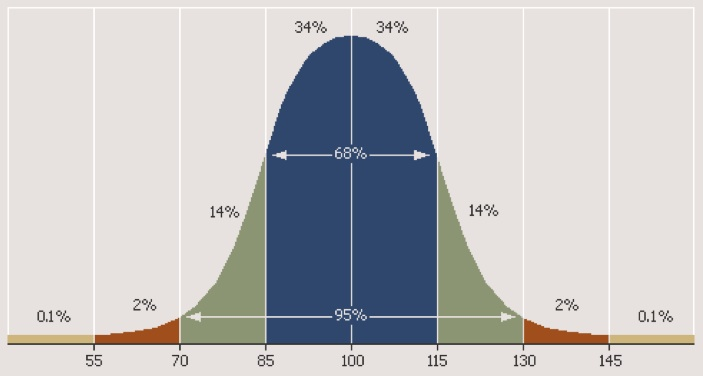
\includegraphics[scale=0.3]{IQ.jpg}
\end{center}
\caption{Gausova raspodela IQ testa}
\label{fig:iqSlika}
\end{figure}

\begin{table}[h!]
\begin{center}
\caption{Klasifikacija na osnovu IQ testa}
\label{tab:tabelaIQ}
\begin{tabular}{|c|c|c|} \hline
IQ Domen & Klasifikacija & Procenat ljudske populacije\\ \hline
(55, 70]& Granična zaostalost & 2\%\\ \hline
(70, 85] & Zatupljenost & 14\%\\ \hline
(85, 115] & Prosečna inteligencija & 68\%\\ \hline
(115, 130] & Visok nivo inteligencije & 14\%\\ \hline
(130, 145] & Veoma visok nivo & 2\% \\ \hline
\end{tabular}
\end{center}
\end{table}


\section{Veštačka inteligencija umesto čoveka}

\subsection{Veštačka inteligencija u saobraćaju}

U poslednjoj deceniji došlo je do značajnog unapredjenja tehnologije samovozećih automobila. Ove nove sposobnosti će imati veliki globalni uticaj koji bi mogao značajno da promeni društvo, a da ne pominjemo značajna poboljšanja koja donose opštoj efikasnosti, pogodnosti i bezbednosti naših puteva i transportnih sistema. Rešavanje problema vezanih za tehnologiju samostalnog upravljanja je važno, posebno imajući u vidu široke potencijalne uticaje. Širom sveta se godišnje pređe 10 triliona automobilskih milja, sa složenim i novim uslovima koji stvaraju milione situacija u kojima bi autonomna vozila mogla da pokvare. Ipak, postoje mnogi izazovi koji ostaju na svim nivoima funkcionalnosti sistema.

Takodje u vodnom saobraćaju, komitet za pomorsku sigurnost Medjunarodne pomorske organizacije (the International Maritime Organization – IMO) je jos 2017. godine prihvatio izazov u pripremi pravnog okvira za uvodjenje autonomnih brodova – brodova bez posade. U pripremi je pravlinik u kojem su već definisana tehnička pravila na osnovu kojih bi oni radili. 

Naravno, takve i slične inovacije nisu česta pojava samo u automobilskoj i brodo-mašinskoj industriji. Danas možemo čuti i za avione kojima pilotira veštačka inteligencija i mnoga druga prevozna sredstva kojima će u budućnosti upravljati roboti.

Pomoću AI prevozna sredstva će postati mnogo efikasnija, imaće povećani kapacitet i bolje planiranje ruta. Na primer, često se dešava da vozovi do odredišta stižu puni a vraćaju se prazni. Ovo je jako štetno za ekonomiju i životnu sredinu. 

Takodje, ono što je najvažnije, došlo bi do potpune eliminacije ljudske greške. Veliki broj nesreća na putu je prouzrokovan upravo umorom, nepažnjom ili zbog neodgovornosti ljudi. 

\subsection{Veštačka inteligencija u okviru arheološke nauke}

Datiranje predmeta informatičkim sredstvima, postalo je potreba koja se može rešiti samo kompleksnim ekspertnim sistemom. Veštačka inteligencija u službi arheologije pruža široke mogućnosti koje nisu ostvarive klasičnim arheološkim sistemima dokumentovanja i obrade.
Ekspertni sistemi su programi koji manipulišu znanjem iz neke oblasti da bi na kvalitetan način odgovarali na pitanja koja uobičajeno rešavaju ljudi - eksperti. Primene ekspertnih sistema su česte u medicini, hemiji, vojnoj i naftnoj industriji. Međutim, retki su primeri ekspertnih sistema u društvenim naukama, pa i u arheologiji.


\subsubsection{Ekspertni sistem PANDORA i rezultati rada}


U ovom trenutku, ekspertni sistem PANDORA poseduje oko 600 pravila o rimskim lampama. Kvalitet odgovora koji daje PANDORA, kada su joj dostupni relevantni podaci, je na nivou arheologa eksperta koji se bavi ovom oblašću. Istovremeno, PANDORA je u stanju i da postavlja,
u odnosu na literaturu, samostalne hipoteze o datiranju iskopina. Na svakom koraku izvođenja, PANDORA na zahtev korisnika nudi objašnjenje u vezi istorije rada, odnosno razloga za neki postupak. Multimedijalne pogodnosti, prikazivanje slika, video i zvučnih zapisa, kao i svojevrsna baza podataka znatno brže dovode do relevantnih podataka, nego što je to slučaj sa klasičnim tekstom. Pored toga, nezavisnost baze znanja od mehanizma izvođenja dozvoljava da isti program radeći
nad raznim podacima preuzima ulogu eksperata iz raznih oblasti. Sve ovo čini da je PANDORA
pogodna i za uloge konsultanta istraživačima i kao edukativno sredstvo kojim se studentima il-
ustruje rad eksperata. Odgovori koje daje PANDORA su implicitno sadržani u znanju, odnosno pravilima u bazi znanja. U tom smislu, PANDORA ne može ponuditi ništa
što joj na posredan način nije unapred ugrađeno. Ali, PANDORA sistematski provera mogućnosti
i može doći do odgovora koje bi čovek prevideo zbog velikog obima raspoloživog znanja. Na taj
način PANDORA može davati odgovore koji do sada nisu ponuđeni u stručnoj literaturi.


\subsection{Veštačka inteligencija u psihijatriji}

Mnogi tvrde da će AI transformisati tehničke aspekte psihijatrije. Na primer, tehnologija pametnog telefona omogućava prikupljanje podataka, čija analiza obećava znatno poboljšanu karakterizaciju bolesti i njihovih putanja. Takve metode su već pokazale potencijal u predviđanju recidiva kod bipolarnog poremećeja. Zajedno sa poboljšanim modelima lečenja efikasnost i sve prirodnije taksonomije mentalnih bolesti zasnovane na podacima, čini se verovatno da će kompjuteri u dijagnozi i planiranju lečenja uskoro nadmašiti ljude.\\
AI još uvek nije u stanju da razgovara sa dovoljno fleksibilnosti da bi održao psihijatrijski intervju. Međutim, obrada prirodnog jezika brzo napreduje i konverzacijski agenti su već našli primenu u proceni navika konzumiranja alkohola. Zaista, postoje jaki dokazi koji sugerišu da ljudi mogu da izgrade terapeutske veze sa agensima veštačke inteligencije. Dokazi sugerišu da ljudi mogu biti iskreniji prema računarima nego prema ljudima. Čini se vrlo verovatno da će ljudi lako doživeti AI kliničara kao istinski brižnog i razumevajućeg. Uz dovoljno podataka, buduća AI će izgraditi dovoljno dubok model odgovora osobe da njeno razumevanje njih prevazilazi razumevanje njihovog psihijatra.\\
Možda će ljudski pacijenti želeti ljudske lekare, sa svim njihovim čudnostima i komparativnom nesposobnošću, jednostavno zato što su ljudi. Cinično, ako su silicijumski psihijatri jeftiniji i merljivo efikasni kao ljudski psihijatri, mogli bi naći masovno zaposlenje samo na osnovu ekonomskih zahteva. Još pozitivnije, AI obećava značajne prednosti za pacijente. Umesto da složene pojedince svrstava u dijagnostičke kategorije i da dodeljuje tretmane zasnovane na generičkim smernicama, AI nudi zaista individualizovanu negu. Štaviše, za razliku od veoma fragmentiranih puteva nege kojima su pacijenti trenutno izloženi, lični AI kliničar bi bio dostupan manje-više bilo gde (od primarne nege do odeljenja za pacijente), u bilo koje vreme. Vremenom bi se tada moglo zaraditi i održati poverenje pacijenata. Stoga, ljudi mogu smatrati da je briga vođena veštačkom inteligencijom humanija od statusa današnje psihijatrije; u svojoj želji da budu shvaćeni i tretirani na osnovu najboljeg naučnog razumevanja, oni će voljno izabrati AI umesto njegove alternative od krvi i mesa.



\section{Zašto veštačka inteligencije \textit{ne može} da zameni čoveka}	
\label{poglavlje:ton}
Začetna ideja veštačke inteligencije: da svaki aspekat učenja, ili drugi oblik inteligencije, može biti do tančina opisan, tako da računar može da ga \emph{imitira}\cite{mitedu}; je danas, pola veka kasnije, ostala samo ideja. Modeli veštačke inteligencije su uglavnom kreirani tako da značajno nadmaše ljudske sposobnosti u poslu koji obavljaju\cite{floridi} (npr. automatizovano igranje igara). U budućnosti se teži da mašine ispoljavaju ovakvu superiornost ne samo u jednoj disciplini, i da razviju mogućnost introspekcije. Teško je sa sigurnošću tvrditi šta će se dogoditi, ali u predvidivoj budućnosti se ovakve težnje smatraju nemogućim \cite{fjelland}. 

\subsection{Uska veštačka inteligencija}
U prethodnom je ključno primetiti da se mašina osposobljava \emph{za određeni posao}, u kom njene mogućnosti značajno nadmašuju ljudske. Ovakva pristup se zove Uska veštačka inteligencija (\emph{eng} Artificial Narrow Intelligence); i to je \textbf{jedini} do sada implementiran oblik veštačke inteligencije. UVI je značajno unapredila kvalitet života ljudi, automatizacijom poslova koje je čovek do sada obavljao, ali mnogo sporije i sa manjom preciznošću. Samo neki od primera su: vremenska prognoza, prepoznavanje lica sa nadzornih kamera, predviđanje cena na berzi,\dots\\

Suštinski, ono što veštačku inteligenciju izdvaja od ostalih oblasti računarstva, jeste automatizacija ljudskog ponašanja koje bi kod pojedinca bilo okarakterisano kao \emph{inteligentno}. Sam čin automatizacije je ono što računarstvo čini značajnim, i ne treba se bojati računara koji je pobedio Kasparova, ništa više nego kalkulatora.\\

\subsection{Generalna veštačka inteligencija}
Možda realnija od pomenutih težnji, u razvoju veštačke inteligencije, je Generalna veštačka inteligencija (\emph{eng} Artificial General Intelligence). Ideja je da jedna mašina, poput čoveka, ispoljava višestruko inteligentnu prirodu \ref{ljudskaInt:definicije}. Generalno inteligentan sistem bi svoju kreativnost realizovao kreiranjem slike na osnovu zadatog opisa \footnote{Poput DALL-E 2 modela, kompanije Open AI} \cite{dalle2}, a matematičko-logičku inteligenciju ispoljio (\textbf{samoukim}) rešavanjem zadataka sa Internacionalne matematičke olimpijade \cite{formalmath}, i na ostale nadljudkse načine. Iako su ovakva dostignuća čoveku nezamisliva, ona se svode na integraciju usko inteligentnih modela, što možda i nije toliko revolucionarno koliko sama ideja generalne veštačke inteligencije zvuči. Najveći izazov bi bio uspešna integracija ovako kompleksnih i trenažno-vremensko-energetski zahtevnih modela u jedan sistem. Koliko god banalno zvučao, realizacija ovog izazova bi za čoveka bio mnogo veći uspeh, nego izvršavanje pomenutih zadataka od strane mašine.

\subsection*{Nedostatak inteligencije kod inteligentnih mašina}
Koliko god jedan ,,inteligentan" model bio brz, inovativan i precizan u svojim predviđanjima; on i dalje može jedino da previdi \emph{šta} će se dogoditi, a ne \emph{kako} ili \emph{zbog čega}. Očigledno je odsustvo inteligencije u ovakvom sistemu, ukoliko se podsetimo Termanove definicije \ref{ljudskaInt:definicije}. Osim \emph{razumevanja} koncepata, Terman zahteva i njihovo \emph{kreiranje}. Kod revijalnih modela veštačke inteligencije, sva inovativnost potiče od čoveka - modeli u najboljem slučaju maskiraju samu realizaciju. I bez definicija, \emph{intuitivno} je jasno da nemogućnost da se uoči uzročna veza, značajno ugrožava intelektualnu karakterizaciju nekog sistema. \\
Možda, ali samo na kratko, nas sve veća upotreba transformatora (\emph{eng} Transformers) može navesti da pomislimo da je u tom slučaju Sternova \ref{ljudskaInt:definicije} definicija zadovoljena; međutim, resursi koje transformatori koriste - osim što u potpunosti zavise od čoveka (Nauka o istraživanju podataka, \emph{eng} Data Science) - troše i daleko više energije, za obavljanje najobičnijih zadataka\cite{frontiers} (poput prepoznavanja lica).\\

Teoriju višestruke inteligencije je u kontekstu mašina suvišno i komentarisati, obzirom da su motoričke, perceptivne, intra i introspektivne sposobnosti još uvek van dosega i najpametnijeg modela veštačke inteligencije.


\section{Zaključak}
\label{sec:zakljucak}

Na osnovu svih ovih informacija koje smo iskazali do sada, mi bi smo trebali da dodjemo do zaključka da li Veštačka Inteligencija može da zameni ljudsku inteligenciju ili ne? Neka definicija Veštačke inteligencije bi mogla izgledati ovako: Veštačka inteligencija je inteligencija koju pokazuje mašina. Zapravo, ona ima sposobnost da primi informacije iz spoljašnje sredine, da ih procesuje i da na osnovu njih na neki način autonomno rezonuje, pre svega, sugestije za čoveka kako da unapredi nešto ili koja je, na primer, dijagnoza u medicini.\\
Kao što se i da primetiti na osnovu svega prethodnog, odgvor na ovo pitanje nije uopšte lako naći. A glavni razlog, leži u tome sto su mišljenja podeljena. Veliki broj ljudi bi rekli da može, a sa druge strane isto tako veliki broj ljudi bi rekli da ne može. Samim tim, naša tema se deli na dva dela. Pripadnici onih koji misle da Veštačka Inteligencija može da zameni ljudsku, kao svoj glavni argument kažu, da roboti mogu da rade sve isto kao i ljudi samo još bolje i na višem nivou. Kako se tehnologija više razvija iz dana u dan, roboti su sve sposobniji i sposobniji. Oni danas mogu da rešavaju teške probleme, donose neke važne odluke i neprestano uče i razvijaju se do beskonačnosti. Danas primena veštačke inteligencije se može naći gde god. Mi smo spominjali primenu veštacke inteligencije u saobraćaju, i to kako se danas sve više i više radi na tome, da se što veći broj vozila kontrolise bez obaveznih vozača, pilota, kapetana... Takodje svakodvnevna upotreba Veštačke inteligencije u saobraćaju koju mi možda ni ne primetimo, su razne mape grada, u kojima Veštačka inteligecija računa koji je najbrži put od nas do našeg cilja. Postoje razni drugi primeri svakodnevne veštačke inteligencije o kojima mi uopšte nismo ni svesni. Samim tim što veštačka inteligencija ima tako širok dijapazon radnji i poslova koje može da obavlja, to nas dovodi do jednih od glavnih argumenata pripadnika koji su protiv Veštačke inteligencije, a to je masovno gubljenje radnih mesta. Danas kada dođete u restoran brze hrane koji ima prozor za vozače, vašu porudžbinu prima i unosi u čovek zaposlen u restoranu. Mislim da za pet godina postoji dobra šansa da ta osoba više neće imati taj posao, da će ga obavljati kompjuter koji može da razume šta vi govorite i primi vašu narudžbinu.\\
Ako bi Veštačka Inteligencija zamenila čoveka u rutniskim poslovima, bilo bi ugašeno oko 65 miliona poslova (Svetski Ekonomski Forum), ali i samim tim bilo bi otvoreno 85 miliona novih. Pri čemu opet dolazimo do konflikta da li je u redu, zameniti žive ljude robotima. Jedan od glavnih razloga zašto neki misle da Veštačka inteligencija niked neće zameniti ljudsku ma koliko god ona bila brža, bolja i naprednija od naše, je to sto VI može da razume neki koncept, kako on radi, i šta će on prouzrokovati, ali ne može da razume zbog čega je to tako. Takodje ljudi misle da postoji veliki broj poslova gde VI neće moći da zameni ljudsku zato što joj fali „ljudskosti“. Robot nikad neće moći da stvarno oseća tugu, sreću, radost, mržnju...

\begin{thebibliography}{9}

\bibitem{turing2009computing} Alan M. Turing. \emph{Parsing the turing test}. Springer - Dordrecht, 2009.

\bibitem{terman}Terman, L. M. \emph{Intelligence and its measurement: A symposium}. Journal of Educational Psychology, 1921.

\bibitem{Gardner1993-ps} Gardner H., \emph{Frames of mind : the theory of multiple intelligences}, 1993.

\bibitem{stern} Stern, William, and Anna Trans Barwell. \emph{Psychology of early childhood: Up to the sixth year of age, rev. and enlarged}, 1924.

\bibitem{mitedu}Dick, S. \emph{Artificial Intelligence} Harvard Data Science Review, 1(1). https://doi.org/10.1162/99608f92.92fe150c, 2019.

\bibitem{floridi} Floridi, L. \emph{The fourth revolution: How the info sphere is reshaping human reality}. Oxford: Oxford University Press, 2016.

\bibitem{fjelland}Fjelland, R. \emph{Why general artificial intelligence will not be realized}. Humanit Soc Sci Commun 7, 10 (2020). https://doi.org/10.1057/s41599-020-0494-4

\bibitem{frontiers}Korteling, J.E., Hans, et al. \emph{Human-versus artificial intelligence}. Frontiers in artificial intelligence 4 (2021): 622364.

\bibitem{formalmath} Polu, Stanislas, et al. \emph{Formal mathematics statement curriculum learning.} arXiv preprint arXiv:2202.01344 (2022).

\bibitem{dalle2} Ramesh, Aditya, et al. \emph{Hierarchical text-conditional image generation with clip latents}. arXiv preprint arXiv:2204.06125 (2022).


\end{thebibliography}

\end{document}
